\begin{frame}

\frametitle{OpenGL}

OpenGL is a graphics API (similar in scope to Direct3D) that allows to use the
graphics card to draw 2D and 3D vector graphics.

\begin{itemize}
    \item{1992 - OpenGL is first released}
    \item{2004 - OpenGL 2.0 is released. Adds support for programmable pipeline (shaders).}
    \item{2010 - OpenGL 4.0 is released. Adds support for geometry shader (tesselation).}
\end{itemize}

\begin{center}
    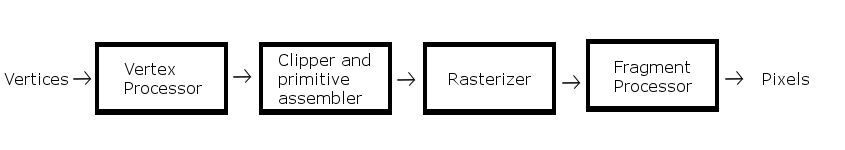
\includegraphics[width=\textwidth]{images/pipeline.png}
\end{center}

\end{frame}

% ---------------------------------------------------------------------

\begin{frame}[fragile]

\frametitle{Old method for drawing}

\begin{center}
\begin{lstlisting}
glColor3f(1.0f, 0.0f, 0.0f);
glBegin(GL_QUADS);
    glVertex2f(-0.25f, 0.25f);
    glVertex2f(-0.5f, -0.25f);
    glVertex2f(0.5f, -0.25f);
    glVertex2f(0.25f, 0.25f);
glEnd();
\end{lstlisting}
\end{center}

Moreover the API had to support many features, for example textures coordinates,
lighting, shadows, coordinate transformation and perspective matrices.
\newline
\\
This results in a complex API and lack of flexibility.

\end{frame}

% ---------------------------------------------------------------------

\begin{frame}[fragile]

\frametitle{Modern approach}

\begin{itemize}
    \item{Allow management of GPU memory from host CPU.}
    \item{Programmable pipeline with shaders.}
\end{itemize}

\vspace{5mm}
\textbf{Advantages}: great flexibility, reduced complexity of API and driver implementations
\newline
\\
\textbf{Disadvantages}: lots of boiler-plate code, not noob-friendly

\end{frame}

% ---------------------------------------------------------------------

\begin{frame}[fragile]

\frametitle{OpenGL state machine}

Since the rendering of the 3D scene is a very complex task, OpenGL uses
the concept of state machine to simplify the API interface (avoid function
with too many arguments).

\begin{center}
\begin{lstlisting}
// Tell OpenGL which array contains the data
glBindBuffer(GL_ARRAY_BUFFER, vbo);
// Specify how the data for position can be accessed
glVertexAttribPointer(0, size, GL_FLOAT, GL_FALSE, 0, 0);
// Enable the attribute
glEnableVertexAttribArray(0); // location = 0

// Draw
glDrawArrays(type, 0, vertex_num);
\end{lstlisting}
\end{center}

\end{frame}

% ---------------------------------------------------------------------

\begin{frame}[fragile]

\frametitle{OpenGL VBOs}

VBO (Vertex Buffer Object) - is an array of data in the GPU memory for storing vertices.

\vspace{5mm}

\begin{lstlisting}
// Tell OpenGL we want to allocate array
glGenBuffers(1, &vbo);
/* Tell OpenGL we want to modify the state
    of the following array */
glBindBuffer(GL_ARRAY_BUFFER, vbo);

// Actually allocate memory
glBufferData(GL_ARRAY_BUFFER, size,
    NULL, GL_DYNAMIC_DRAW);

// Tell OpenGl we are done with the array
glBindBuffer(GL_ARRAY_BUFFER, 0);
\end{lstlisting}

\end{frame}

\begin{frame}[fragile]

\frametitle{OpenGL Textures}

Texture - is an image that is mapped to vertices.

\begin{center}
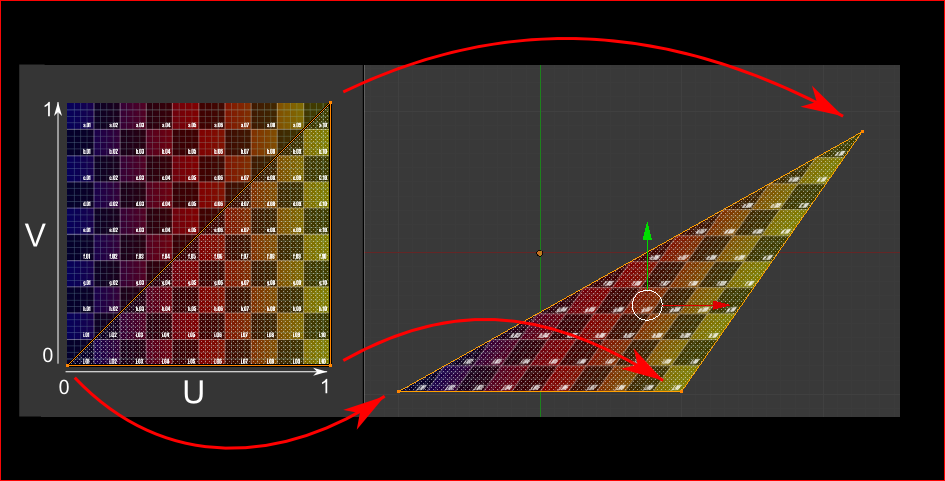
\includegraphics[width=\textwidth]{images/uv.png}
\end{center}

\end{frame}

% ---------------------------------------------------------------------

\begin{frame}[fragile]

\frametitle{OpenGL Textures}

\begin{lstlisting}[basicstyle=\fontsize{7pt}{8pt}\ttfamily]
// Tell OpenGl we want to allocate a texture
glGenTextures(1, &texture);
/* Tell OpenGl we are going to modify the state
    of the following texture */
glBindTexture(GL_TEXTURE_2D, texture);

// Set interpolation method to linear
glTexParameteri(GL_TEXTURE_2D, GL_TEXTURE_MIN_FILTER, GL_LINEAR);
glTexParameteri(GL_TEXTURE_2D, GL_TEXTURE_MAG_FILTER, GL_LINEAR);

// Actually allocate memory
glTexImage2D(GL_TEXTURE_2D, 0, GL_RGBA8, width, height,
    0, GL_RGBA, GL_UNSIGNED_BYTE, NULL);    

// Tell OpenGl we finished modifying this etxture
glBindTexture(GL_TEXTURE_2D, 0);
\end{lstlisting}


\end{frame}


% ---------------------------------------------------------------------

\begin{frame}[fragile]

\frametitle{OpenGL shaders}

Shaders \textrightarrow $\,$ programs that run on the GPU (analogous to CUDA kernels).
\newline
\\
Three types:
\begin{itemize}
    \item{Vertex shader - transforms vertex coordinates.}
    \item{Fragment shader - transforms pixel colors.}
    \item{Geometry shader - can add vertices.}
\end{itemize}

\begin{center}
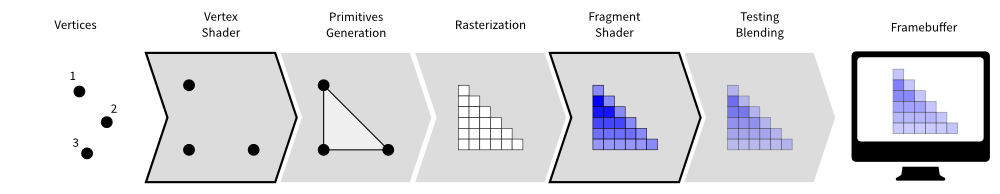
\includegraphics[width=\textwidth]{images/shaders.png}
\end{center}

\end{frame}
% ---------------------------------------------------------------------

\begin{frame}[fragile]

\frametitle{Vertex shader}

\begin{lstlisting}
#version 330

layout(location = 0) in vec2 position;
out vec2 texCoord;

void main() {
    texCoord = vec2(position.x/2 + 0.5, position.y/2 + 0.5);
    gl_Position = vec4(position.x, position.y, 1.0, 1.0);
}
\end{lstlisting}

\end{frame}
% ---------------------------------------------------------------------

\begin{frame}[fragile]

\frametitle{Fragment shader}

\begin{lstlisting}[basicstyle=\fontsize{7pt}{8pt}\ttfamily]
#version 330

uniform sampler2D tex;
in vec2 texCoord;
out vec4 colorOut;

void main() {
    float strength = texture(tex, texCoord).x;

    // Colormap
    //   1     red      (1, 0, 0)
    //   0.75  yellow   (1, 1, 0)
    //   0.5   green    (0, 1, 0)
    //   0.25  cyan     (0, 1, 1)
    //   0     blue     (0, 0, 1)
    // RED
    float red = (strength > 0.75) ?
        1 : ((strength > 0.5) ?
            (strength - 0.5) * 4 : 0);
    // GREEN
    float green = (strength <= 0.75 && strength > 0.25) ?
        1 : ((strength > 0.75) ? 1 - strength : strength) * 4;
    // BLUE
    float blue = (strength > 0.5) ?
        0 : ((strength > 0.25) ?
            (0.5 - strength) * 4 : 1);

    colorOut = vec4(red, green, blue, 1);
}
\end{lstlisting}

\end{frame}
% ---------------------------------------------------------------------

\begin{frame}[fragile]

\frametitle{How to draw}

\begin{lstlisting}
// Select texture unit
glActiveTexture(GL_TEXTURE0);
// Use this texture
glBindTexture(GL_TEXTURE_2D, texture);

// Assign texture unit index to the fragment shader
glUniform1i(1, 0); // location = 1, texture unit = 0

/*** We need a support to draw our texture ***/
// Tell OpenGL which array contains the data
glBindBuffer(GL_ARRAY_BUFFER, vbo);
// Specify how the data for position can be accessed
glVertexAttribPointer(0, 2, GL_FLOAT, GL_FALSE, 0, NULL);
// Enable the attribute
glEnableVertexAttribArray(0); // location = 0

// Draw
glDrawArrays(GL_TRIANGLE_STRIP, 0, 4);

// Disable array and texture
glBindBuffer(GL_ARRAY_BUFFER, 0);
glBindTexture(GL_TEXTURE_2D, 0);
\end{lstlisting}

\end{frame}
% ---------------------------------------------------------------------

\begin{frame}[fragile]

\frametitle{OpenGL-CUDA interperability}

\end{frame}
% ---------------------------------------------------------------------

\begin{frame}[fragile]

\frametitle{OpenGL-CUDA interoperability}

\end{frame}

% ---------------------------------------------------------------------

\begin{frame}[fragile]

\frametitle{Execution model}


\end{frame}
% ---------------------------------------------------------------------

\begin{frame}[fragile]

\frametitle{Registering and mapping}


\end{frame}


% Brief into to opengl
% Intro
% Advantages - Disadvantages
% Execution model
% Registering and Mapping
% State machine
% Arrays and Textures
% Shaders
% Drawing
% Show code
